\paragraph{Example}
Particle in 2D with potential $V(x,y)$:
$$L = \frac{1}{2}m(\dot{x}^2 + \dot{y}^2)-V(x,y)$$
$$\frac{d}{dt}\left( \frac{\partial L}{\partial \dot{x}} \right) = \frac{\partial L}{\partial x}$$
I.e.
$$m\ddot{x} = -\frac{\partial V}{\partial x}$$
$$m\ddot{y} = -\frac{\partial V}{\partial y}$$
In polar ($x=r\cos \theta$, $y=r\sin \theta$):
$$\dot{x} = \dot{r} \cos \theta - r\dot{\theta} \sin \theta$$
$$\dot{y} = \dot{r} \sin \theta + r\dot{\theta} \cos \theta$$
In Newtonian formalism we'd need $\ddot{x}$, which is often not trivial.

$$\dot{x}^2 + \dot{y}^2 = (\dot{r} \cos \theta - r\dot{\theta} \sin \theta)^2 + (\dot{r} \sin \theta + r\dot{\theta} \cos \theta)^2 = \dot{r}^2 + r^2 \dot{\theta}^2$$
Now
$$L(r,\dot{r},\theta,\dot{\theta}) = \frac{1}{2}(\dot{r}^2+r^2\dot{\theta}^2) - V(r, \theta)$$
Differentiating:
$$m\ddot{r} = mr\dot{\theta}^2 - \frac{\partial V}{\partial r}$$
$$2mr\dot{r}\dot{\theta} + mr^2 \ddot{\theta} = - \frac{\partial V}{\partial \theta}$$
\subsection{Constraints}
In some problem we have forces that constrain the movement of body. For example, movement on rope is 1D even though it happens in 3D. Rigid body keeps distance between its points constant. Molecules in the room are constrained to stay in the room. 
\paragraph{Holonomic constrains}
Constrain is called holonomic if it can be described with function
$$C(\vec{r}_1,\dots,\vec{r}_n, t) = 0$$

So if we have a bead on rope:
$$x^2+y^2=0$$
Or, for rigid body;
$$(x_2-x_1)^2 + (y_2-y_1)^2 = r_{12}^2$$
However, molecules in the room is non-holonomic constrain:
$$-L \leq x \leq L$$
\paragraph{bead on rotating rope}
Let's describe a particle sitting on a particular point on a bead.


\begin{center}
	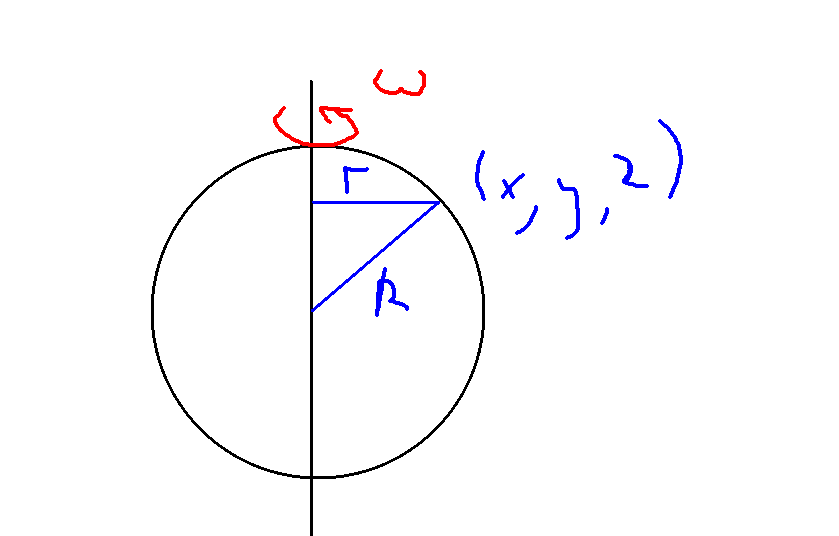
\includegraphics[width=0.5\linewidth]{./lect4/1.png}
\end{center}
We have two constraints. First is that particle on a sphere:
$$x^2+y^2+z^2-R^2 = 0$$
Second is that it doesn't move
$$(x,y,z) = (r\sin \omega t, r\cos \omega t, z) \Rightarrow x\cos \omega t - y\sin \omega t = 0$$

\subsubsection{Solving problems with constrains}
Given problem with $n$ degrees of freedom and $m$ constrains.

If $x_1, \dots, x_n$ are initial degrees of freedom.
and
$$\begin{cases} c_1(x_1, \dots, x_n, t) = 0 \\ \dots \\ c_m(x_1, \dots, x_n, t) = 0 \end{cases}$$

Effectively we have $n-m$ degrees of freedom. With movement equation
$$m\ddot{r} = \underbrace{F^i}_{Potential forces} + \underbrace{f^i}_{Constraining forces}$$